\documentclass[conference]{IEEEtran}
\usepackage{cite}
\usepackage{amsmath,amssymb}
\usepackage{graphicx,booktabs,makecell}
\usepackage{algorithm,algpseudocode}
\usepackage[hidelinks]{hyperref}
\begin{document}
\title{Combining Instance Filtering and Attribute Weighting in Decision Tree and Na\"ive Bayes Hybrids: An Experimental Study}
\author{
\IEEEauthorblockN{Ikramul Hasan Moral}
\IEEEauthorblockA{Dept. of CSE\\
United International University\\
Dhaka, Bangladesh\\
imoral223489@bscse.uiu.ac.bd}
\and
\IEEEauthorblockN{Dr. Dewan Md. Farid}
\IEEEauthorblockA{Professor, Dept. of CSE \& Director, MSCSE Program\\
United International University\\
Dhaka, Bangladesh\\
dewanfarid@cse.uiu.ac.bd}}


\maketitle
\begin{abstract}
A published family of hybrid classifiers cleans training data in two ways: a
Na\"ive Bayes model removes training rows that it misclassifies, and a decision
tree selects attributes and gives them weights for Na\"ive Bayes. We rebuilt
both cleaning steps and every way of combining them: each step on its own, both
steps in either order, and both steps applied to separate copies of the training
data and then merged. We evaluated ten public datasets with ten repetitions of
stratified 10-fold cross-validation, redid every cleaning step inside each
training fold, and scored every held-out row. Our main findings are negative and
consistent. Plain C4.5 averaged 86.33\% accuracy, and every design that removed
instances landed about five points below it, no matter how the steps were
arranged. Weighting attributes alone raised Na\"ive Bayes from 75.93\% to
77.35\%, the largest gain any cleaning design made over its base classifier, but
even that difference is not statistically significant. None of the sixteen paired comparisons, on
accuracy or on macro-averaged F1, was significant after Holm correction; the
smallest adjusted p-value was 0.44. When we instead cleaned once before
cross-validation, the scores of the filter-based designs rose by 13.5 to 16.5
points, because the cleaning step had already seen the test rows and had removed
difficult cases from the evaluation. Deletion also fell unequally on the
classes: on breast cancer the plain filter removed 50.63\% of recurrence-event
rows but only 14.51\% of the rest. We conclude that combining these two cleaning
steps does not improve accuracy under a fair evaluation, and we recommend
cleaning inside the training fold, reporting what was deleted, and checking
which classes lost training rows.
\end{abstract}
\begin{IEEEkeywords}
Na\"ive Bayes, decision tree, data cleaning, instance filtering, attribute
weighting, cross-validation
\end{IEEEkeywords}

\section{Introduction}
Farid et al.~\cite{farid2014hybrid} published two hybrid classifiers for
multi-class classification. The first cleans training data with Na\"ive Bayes
(NB): it fits NB on the training rows, removes the rows whose predicted label
disagrees with the supplied label, and fits a decision tree on the rows that
remain. The second cleans the attributes: it fits a decision tree, keeps the
attributes that the tree tests, gives a larger weight to attributes used nearer
the root, and fits NB on the weighted attributes. A natural question follows:
if each step helps on its own, does using both together help more, and does the
order matter?

This paper answers that question with a controlled experiment. We rebuilt both
published steps from their descriptions, using the same tools (Weka's C4.5
implementation~\cite{witten2016weka} and a textbook NB), and we tested twelve
settings on ten public datasets: the two plain classifiers, each cleaning step
on its own with either final classifier, both steps in either order with either
final classifier, and a parallel design in which the two steps act on separate
copies of the same training fold and the two cleaned copies are merged into one
training set. Every setting was evaluated with ten repetitions of stratified
10-fold cross-validation, with all cleaning redone inside each training fold and
every held-out row scored.

The experiment produced five findings that we state here and support in
Section~IV.
\begin{enumerate}
\item Our rebuild is sound: the plain classifiers land close to the averages of
the corresponding 2014 tables, within 2.81 points for C4.5 and 1.40 points for
NB.
\item Removing instances is the damaging step. All four designs that remove
instances and end in a tree score about five points below plain C4.5 (80.89\%
to 81.21\% against 86.33\%), whether the removal runs alone, first, second, or
in parallel with the attribute step.
\item The order of the two steps and the choice to chain them at all do not
change the outcome. Swapping the order moves the mean by at most 0.71 points,
and chaining is never better than running the two steps separately.
\item Weighting attributes alone gives the largest gain over its base
classifier: 77.35\% for weighted NB against 75.93\% for plain NB. The gain does
not survive combination, and it is not statistically significant either
($p=0.131$).
\item Cleaning before cross-validation inflates every filter-based score by
13.5 to 16.5 points. The inflated numbers measure which rows the filter
removed, not better classification.
\end{enumerate}
A sixth observation concerns what the filters delete: deletion falls unequally
on the classes, and removing instances first changes which attributes the tree
selects. Section~\ref{sec:deletion} reports this in detail.

\section{The Two Cleaning Steps and How We Combined Them}
\subsection{Removing instances with Na\"ive Bayes}
Given training data $D$, this step fits NB on $D$, predicts the label of every
training row, and keeps a row only when the prediction agrees with the supplied
label. The final classifier, NB or C4.5, is then fitted on the retained rows.
One safety rule is in force: if deletion would leave fewer than two classes,
the step keeps the original training rows instead. Our runs never triggered
this rule.

The rule behind the step is disagreement, not proof of error. A row can be
rejected because its label is wrong, but also because the class distributions
overlap or because NB does not suit the data. We therefore report which rows
were removed rather than calling them noise.

\subsection{Selecting and weighting attributes with a decision tree}
This step fits a C4.5 tree on the training data and reads two things from it:
which attributes the tree tests, and how near the root each attribute is used.
Let $d_j$ be the smallest depth at which the tree tests attribute $j$, counted
with the root at depth one. The weight is
\begin{equation}
\label{eq:weight}
 w_j = \begin{cases}1/\sqrt{d_j}, & j\text{ is tested by the tree},\\
                    0, & \text{otherwise}.\end{cases}
\end{equation}
Attributes with weight zero are dropped. The weighted NB score for class $c$ is
\begin{equation}
\label{eq:score}
 s_c(x)=\log P(c)+\sum_{j}w_j\log P(x_j\mid c),
\end{equation}
and NB predicts the class with the largest score. Equation~\eqref{eq:weight}
makes attributes tested near the root count more, and
Equation~\eqref{eq:score} applies those weights inside NB.

\subsection{The combined designs}
Algorithm~\ref{alg:combined} shows the two sequential designs. The
\emph{instances first} design runs the NB removal step, then fits the selection
tree on the retained rows; the \emph{attributes first} design selects and
weights attributes on the original training fold, then runs the removal step
with weighted NB. In the attributes-first design the same weights
(Equation~\eqref{eq:weight}) are used by the filtering model and by the final
NB; they are not estimated again after deletion. When the final classifier is
C4.5, the weights drop out (a tree does not use them) and only the selected
columns carry over.

\begin{algorithm}[t]
\caption{A combined cleaning design with final learner $L$}
\label{alg:combined}
\begin{algorithmic}[1]
\Require Training data $D$, design $o$, final learner $L\in\{\text{NB},\text{C4.5}\}$
\If{$o=$ instances first}
 \State $D\gets\Call{RemoveInstances}{D,\text{plain NB}}$
 \State $(S,W)\gets\Call{SelectAttributes}{D,\text{C4.5}}$
\Else
 \State $(S,W)\gets\Call{SelectAttributes}{D,\text{C4.5}}$
 \State $D\gets$ the columns $S$ of $D$
 \State $D\gets\Call{RemoveInstances}{D,\text{NB weighted by }W}$
\EndIf
\If{$o=$ instances first}
 \State $D\gets$ the columns $S$ of $D$
\EndIf
\State Fit $L$ on $D$ (NB uses the weights $W$)
\end{algorithmic}
\end{algorithm}

The parallel design leaves out the chaining. It runs the NB removal step on one
copy of the training fold and the selection step on a second copy, both fitted
on the original data, and keeps the rows and the columns that the two copies
accept. The final classifier is then fitted on that merged set; the final NB
uses the tree's weights. This design answers a practical question: if chaining
the two steps is supposed to help, the combined design should at least beat
doing both separately.

If the selection tree tests no attribute, the design keeps all current columns
with unit weights. No such event occurred in our runs. At prediction time the
test rows keep the selected columns, and every held-out row is scored.

\section{Experimental Setup}
\subsection{Data}
\label{sec:data}
Table~\ref{tab:data} lists the ten public datasets named in the 2014 study,
in the file forms we used. Two of our files differ from the 2014 tables: image
segmentation combines two UCI files, and NSL-KDD uses its 20\% training
file~\cite{tavallaee2009detailed}. Glass and NSL-KDD each contain one fewer
class than the original study lists. The two files allow comparisons on shared
data but not an exact reproduction of the original data preparation.

\begin{table}[t]
\caption{Dataset sizes in the files used for evaluation}
\label{tab:data}
\centering
\begin{tabular}{lrrr}
\toprule
Dataset & Rows & Attributes & Classes \\
\midrule
Breast cancer & 286 & 9 & 2 \\
Contact lenses & 24 & 4 & 3 \\
Diabetes & 768 & 8 & 2 \\
Glass & 214 & 9 & 6 \\
Iris & 150 & 4 & 3 \\
Soybean & 683 & 35 & 19 \\
Vote & 435 & 16 & 2 \\
Image segmentation & 2310 & 19 & 7 \\
Tic-tac-toe & 958 & 9 & 2 \\
NSL-KDD & 25192 & 41 & 22 \\
\bottomrule
\end{tabular}
\end{table}

\subsection{Implementation}
C4.5 is Weka J48 3.8.6 with pruning and default
settings~\cite{witten2016weka}. NB uses add-one counts for nominal attributes
and Gaussian likelihoods for numeric attributes. Attributes stay in their
original columns, so tree selection refers to original attributes and not to
binary indicator columns. The category vocabularies come from the complete
files and stay fixed across folds; a missing nominal value forms its own
category. Counts and distributions are estimated on training rows only.

\subsection{The main evaluation: cleaning inside each training fold}
The main evaluation uses stratified 10-fold cross-validation, repeated ten
times with different random splits, giving 100 folds per dataset and per
setting. All twelve settings share the same splits. Inside every training
fold, the pipeline refits the NB model that removes rows, the tree that selects
attributes, and the final classifier; the held-out fold is then scored with all
of its rows. No test row is ever removed, and no learner setting is tuned.

This evaluation is deliberately strict. The cleaning steps see only the
training rows of the fold they run in, so they cannot borrow information from
the rows they will be scored against.

\subsection{A diagnostic: cleaning once before cross-validation}
For comparison, we also ran a weaker procedure: clean the whole dataset once,
then cross-validate only the final classifier on the cleaned data. This
procedure lets the cleaning step see labels from rows that later end up in test
folds, and, for the designs that remove rows, it also shrinks the set of rows
that will ever be scored. Its scores are reported only as a diagnostic of what
this weaker procedure would exaggerate; they are not performance estimates.

\subsection{Measures and statistical tests}
We report accuracy and macro-averaged F1, the unweighted mean of the per-class
F1 scores over the classes present in a fold. Each dataset's score averages its
100 folds, and the summary gives each dataset equal weight; the spread values
in the tables are standard deviations over the ten repetition-level averages.
For statistical tests we use two-sided Wilcoxon signed-rank tests on the ten
per-dataset averages, with exact permutation enumeration. The comparison
family covers, for each final classifier, the five cleaning settings against
the plain classifier, the two order swaps, and the two
sequential-versus-parallel contrasts, sixteen comparisons in total, each
computed on accuracy and on macro-F1. Holm's correction, which rescales
p-values for the number of tests, is applied across all thirty-two. We chose
this family after seeing the saved results, so the tests are exploratory:
a non-significant result does not prove that two settings are equal.

\section{Results and Findings}
\label{sec:results}
\subsection{No cleaning design beats the plain classifiers}
Table~\ref{tab:summary} shows the main scores and Figure~\ref{fig:change} shows
each cleaning setting's change from its base classifier. Plain C4.5 leads on
both measures, 86.33\% accuracy and 81.92\% macro-F1. The four designs that
remove instances and end in a tree score between 80.89\% and 81.21\%, a loss of
about five points, and the four versions that end in NB stay within half a
point of plain NB (75.42\% to 76.39\% against 75.93\%), with no significant
difference among them. The two designs that only touch attributes, with no row
removal, stay close to their plain classifiers: selecting attributes for C4.5
costs 0.14 points (86.19\% against 86.33\%), and weighting attributes for NB
gains 1.42 points (77.35\% against 75.93\%), the largest gain over a base
classifier in the whole experiment, though not a significant one ($p=0.131$).

\begin{table}[t]
\caption{Main scores (\%): mean $\pm$ standard deviation over the ten
repetition-level averages; each dataset has equal weight}
\label{tab:summary}
\centering
\footnotesize
\setlength{\tabcolsep}{3pt}
% Generated from EXP-E9_farid; 10 datasets, 10 seeds, 10 folds; plain-language labels.
\begin{tabular}{lrr}
\toprule
Method & Accuracy (\%) & Macro-F1 (\%) \\
\midrule
Plain NB (no cleaning) & 75.93 $\pm$ 0.32 & 69.80 $\pm$ 0.52 \\
Plain C4.5 (no cleaning) & \textbf{86.33 $\pm$ 0.33} & \textbf{81.92 $\pm$ 0.44} \\
Remove instances only $\to$ NB & 75.42 $\pm$ 0.46 & 69.08 $\pm$ 0.46 \\
Remove instances only $\to$ C4.5 & 81.03 $\pm$ 0.37 & 75.70 $\pm$ 0.63 \\
Weight attributes only $\to$ NB & 77.35 $\pm$ 0.41 & 71.73 $\pm$ 0.63 \\
Select attributes only $\to$ C4.5 & 86.19 $\pm$ 0.33 & 81.84 $\pm$ 0.42 \\
Instances first, then attributes $\to$ NB & 75.63 $\pm$ 0.45 & 69.60 $\pm$ 0.72 \\
Instances first, then attributes $\to$ C4.5 & 81.21 $\pm$ 0.29 & 75.76 $\pm$ 0.58 \\
Attributes first, then instances $\to$ NB & 76.35 $\pm$ 0.34 & 69.91 $\pm$ 0.60 \\
Attributes first, then instances $\to$ C4.5 & 80.89 $\pm$ 0.45 & 73.93 $\pm$ 0.80 \\
Both steps separately, combined $\to$ NB & 76.39 $\pm$ 0.37 & 70.47 $\pm$ 0.68 \\
Both steps separately, combined $\to$ C4.5 & 81.05 $\pm$ 0.34 & 75.58 $\pm$ 0.58 \\
\bottomrule
\end{tabular}

\end{table}

\begin{figure}[t]
\centering
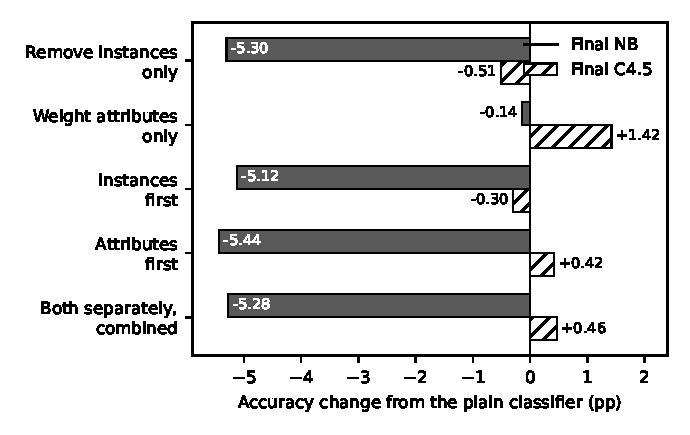
\includegraphics[width=\columnwidth]{figures/accuracy_change_full.pdf}
\caption{Mean accuracy change from the corresponding plain classifier, over
ten datasets with equal weight. Hatched bars end in NB, solid bars in C4.5.
Every design that removes instances loses about five points for the tree;
nothing else moves the means by more than 1.5 points.}
\label{fig:change}
\end{figure}

The per-dataset tables show that the averages hide the worst cases.
Table~\ref{tab:datasets_acc} gives accuracy per dataset. On glass, the
instances-first design with a NB ending falls from 45.95\% to 30.93\%, and the
same design with a C4.5 ending falls from 66.58\% to 48.97\%. On NSL-KDD the
plain tree scores 99.47\% and the removal designs score between 87.07\% and
89.68\%. The single small exception is contact lenses, where the instances-first
NB design improves from 73.00\% to 83.00\%; that dataset has 24 rows, so the
result carries little weight. Table~\ref{tab:datasets_f1} gives the same
picture for macro-averaged F1.

\begin{table*}[t]
\caption{Accuracy by dataset (\%). ``Instances only'' removes training rows
with plain NB and then fits the final classifier; ``Attributes only'' selects
attributes with the tree (NB additionally uses the tree's weights); ``Instances
first'' and ``Attributes first'' chain the two steps in that order; ``Both
separately'' applies the two steps to separate copies of the training fold and
merges them.}
\label{tab:datasets_acc}
\centering
\footnotesize
\setlength{\tabcolsep}{4pt}
% Generated from EXP-E9_farid; 10 datasets, 10 seeds, 10 folds; plain-language labels.
\begin{tabular}{lrrrrrr}
\toprule
Dataset & No cleaning & Instances only & Attributes only & Instances first & Attributes first & Both separately \\
\midrule
breast-cancer & 72.12 & 72.68 & 72.43 & 71.28 & 72.53 & 72.46 \\
contact-lenses & 73.00 & 73.00 & 80.67 & 83.00 & 79.33 & 83.00 \\
diabetes & 75.52 & 74.41 & 76.73 & 75.58 & 75.67 & 75.81 \\
glass & 45.95 & 37.00 & 47.84 & 30.93 & 37.28 & 32.29 \\
image-segmentation & 79.76 & 74.92 & 82.30 & 74.53 & 77.32 & 76.57 \\
iris & 95.53 & 95.33 & 95.40 & 95.33 & 95.87 & 95.60 \\
nsl-kdd & 67.42 & 75.79 & 62.80 & 74.53 & 75.23 & 76.16 \\
soybean & 90.09 & 89.00 & 89.40 & 85.67 & 86.66 & 86.95 \\
tic-tac-toe & 69.83 & 71.89 & 70.68 & 70.03 & 68.07 & 69.72 \\
vote & 90.06 & 90.13 & 95.24 & 95.45 & 95.49 & 95.36 \\
\bottomrule
\end{tabular}
\\[4pt]
% Generated from EXP-E9_farid; 10 datasets, 10 seeds, 10 folds; plain-language labels.
\begin{tabular}{lrrrrrr}
\toprule
Dataset & No cleaning & Instances only & Attributes only & Instances first & Attributes first & Both separately \\
\midrule
breast-cancer & 74.84 & 71.77 & 73.91 & 71.77 & 72.08 & 71.20 \\
contact-lenses & 84.67 & 84.67 & 84.67 & 84.67 & 80.67 & 84.67 \\
diabetes & 74.12 & 75.12 & 74.18 & 75.23 & 75.57 & 74.86 \\
glass & 66.58 & 48.83 & 66.58 & 48.97 & 49.15 & 48.65 \\
image-segmentation & 96.81 & 89.24 & 96.83 & 89.26 & 90.88 & 89.79 \\
iris & 94.27 & 94.93 & 94.27 & 94.93 & 93.80 & 94.93 \\
nsl-kdd & 99.47 & 87.43 & 99.47 & 89.68 & 87.07 & 88.37 \\
soybean & 92.71 & 88.71 & 92.26 & 87.89 & 90.98 & 88.24 \\
tic-tac-toe & 84.74 & 74.43 & 84.74 & 74.55 & 73.17 & 74.43 \\
vote & 95.08 & 95.13 & 95.03 & 95.13 & 95.54 & 95.38 \\
\bottomrule
\end{tabular}

\end{table*}

\begin{table*}[t]
\caption{Macro-averaged F1 by dataset (\%), with the same setting names as
Table~\ref{tab:datasets_acc}.}
\label{tab:datasets_f1}
\centering
\footnotesize
\setlength{\tabcolsep}{4pt}
% Generated from EXP-E9_farid; 10 datasets, 10 seeds, 10 folds; plain-language labels.
\begin{tabular}{lrrrrrr}
\toprule
Dataset & No cleaning & Instances only & Attributes only & Instances first & Attributes first & Both separately \\
\midrule
breast-cancer & 64.42 & 64.22 & 62.57 & 61.33 & 61.57 & 62.94 \\
contact-lenses & 62.31 & 62.31 & 72.27 & 76.47 & 69.87 & 76.47 \\
diabetes & 72.32 & 71.43 & 72.76 & 71.96 & 71.05 & 72.03 \\
glass & 44.98 & 40.72 & 44.71 & 36.78 & 40.42 & 37.99 \\
image-segmentation & 77.78 & 74.52 & 81.42 & 73.40 & 77.06 & 75.82 \\
iris & 95.48 & 95.28 & 95.35 & 95.29 & 95.82 & 95.56 \\
nsl-kdd & 34.06 & 35.87 & 37.58 & 35.36 & 38.18 & 36.46 \\
soybean & 93.13 & 92.59 & 91.33 & 87.27 & 88.40 & 89.95 \\
tic-tac-toe & 63.83 & 64.08 & 64.26 & 62.93 & 61.45 & 62.30 \\
vote & 89.66 & 89.80 & 95.02 & 95.25 & 95.29 & 95.15 \\
\bottomrule
\end{tabular}
\\[4pt]
% Generated from EXP-E9_farid; 10 datasets, 10 seeds, 10 folds; plain-language labels.
\begin{tabular}{lrrrrrr}
\toprule
Dataset & No cleaning & Instances only & Attributes only & Instances first & Attributes first & Both separately \\
\midrule
breast-cancer & 61.81 & 62.68 & 60.52 & 62.65 & 61.37 & 61.82 \\
contact-lenses & 79.47 & 79.47 & 79.47 & 79.47 & 72.27 & 79.47 \\
diabetes & 70.71 & 71.45 & 70.79 & 71.56 & 71.19 & 70.97 \\
glass & 62.00 & 45.29 & 62.00 & 45.45 & 43.35 & 45.03 \\
image-segmentation & 96.81 & 88.96 & 96.83 & 88.98 & 90.79 & 89.53 \\
iris & 94.18 & 94.88 & 94.18 & 94.88 & 93.72 & 94.88 \\
nsl-kdd & 82.25 & 60.33 & 82.92 & 62.05 & 53.18 & 60.82 \\
soybean & 94.26 & 92.08 & 94.10 & 90.47 & 92.08 & 91.21 \\
tic-tac-toe & 82.82 & 66.94 & 82.82 & 67.18 & 66.02 & 66.94 \\
vote & 94.86 & 94.90 & 94.81 & 94.90 & 95.34 & 95.17 \\
\bottomrule
\end{tabular}

\end{table*}

\subsection{Order and combination do not change the outcome}
Table~\ref{tab:tests} lists the paired dataset-level tests. The largest single
difference in the whole family is the attributes-first design's loss to plain
C4.5, $-5.44$ points with raw $p=0.014$; after Holm correction across all
thirty-two tests it stands at $p=0.44$. No other comparison comes closer to
significance, on accuracy or on macro-F1. Swapping the order moves the NB
means by $+0.71$ points ($p=0.275$) and the C4.5 means by $-0.32$ points
($p=0.922$). The sequential designs do not beat doing both separately: all
eight sequential-versus-parallel contrasts lie within 0.76 points on accuracy
and within 1.65 points on macro-F1, and the only raw p-value below 0.05 among
them ($-0.76$ for instances-first against both-separately on NB, $p=0.039$)
does not survive the correction. On this
family of datasets, where the two steps run makes no measurable difference to
accuracy.

\begin{table*}[t]
\caption{Paired dataset-level comparisons. Each difference is the mean over
ten datasets, in percentage points; Holm $p$ is corrected across all
thirty-two tests. No comparison is significant at 0.05 after correction.}
\label{tab:tests}
\centering
\footnotesize
% Generated from EXP-E9_farid; 10 datasets, 10 seeds, 10 folds; plain-language labels.
\begin{tabular}{lrrrrrr}
\toprule
Comparison & Acc.\ diff.\ (pp) & $p$ & Holm $p$ & F1 diff.\ (pp) & $p$ & Holm $p$ \\
\midrule
Remove instances only vs plain C4.5 & -5.30 & 0.055 & 1.000 & -6.22 & 0.164 & 1.000 \\
Select attributes only vs plain C4.5 & -0.14 & 0.562 & 1.000 & -0.07 & 0.938 & 1.000 \\
Instances first vs plain C4.5 & -5.12 & 0.055 & 1.000 & -6.16 & 0.164 & 1.000 \\
Attributes first vs plain C4.5 & -5.44 & 0.014 & 0.438 & -7.99 & 0.037 & 1.000 \\
Both separately vs plain C4.5 & -5.28 & 0.055 & 1.000 & -6.33 & 0.164 & 1.000 \\
Attributes first vs instances first (C4.5) & -0.32 & 0.922 & 1.000 & -1.83 & 0.232 & 1.000 \\
Instances first vs both separately (C4.5) & +0.16 & 0.461 & 1.000 & +0.18 & 0.461 & 1.000 \\
Attributes first vs both separately (C4.5) & -0.16 & 0.770 & 1.000 & -1.65 & 0.193 & 1.000 \\
Remove instances only vs plain NB & -0.51 & 0.652 & 1.000 & -0.71 & 0.232 & 1.000 \\
Weight attributes only vs plain NB & +1.42 & 0.131 & 1.000 & +1.93 & 0.193 & 1.000 \\
Instances first vs plain NB & -0.30 & 1.000 & 1.000 & -0.19 & 0.557 & 1.000 \\
Attributes first vs plain NB & +0.42 & 0.846 & 1.000 & +0.11 & 0.922 & 1.000 \\
Both separately vs plain NB & +0.46 & 0.695 & 1.000 & +0.67 & 0.846 & 1.000 \\
Attributes first vs instances first (NB) & +0.71 & 0.275 & 1.000 & +0.31 & 0.492 & 1.000 \\
Instances first vs both separately (NB) & -0.76 & 0.039 & 1.000 & -0.86 & 0.055 & 1.000 \\
Attributes first vs both separately (NB) & -0.05 & 0.770 & 1.000 & -0.56 & 0.846 & 1.000 \\
\bottomrule
\end{tabular}

\end{table*}

\subsection{Cleaning before cross-validation inflates the filter scores}
Table~\ref{tab:protocols} compares the two procedures for the ten cleaning settings. When the cleaning steps
run once on the full dataset before cross-validation, every design that removes
rows gains 13.50 to 16.51 points over its score under the main evaluation. The
designs that only touch attributes gain 0.72 and 0.33 points. The reason is
mechanical rather than informative. Cleaning before the split gives the NB
model access to labels from rows that later fall in test folds, and, for the
row-removing designs, it deletes rows that the main evaluation would have
scored. The larger numbers therefore describe an easier task on a smaller
sample. This is the pattern to watch for when a published pipeline reports its
cleaning gains without stating where the cleaning ran.

\begin{table}[t]
\caption{Mean accuracy (\%) under the main evaluation (cleaning inside each
training fold) and under the diagnostic (cleaning once before
cross-validation). The difference is descriptive; the diagnostic changes both
the information available and the rows being scored.}
\label{tab:protocols}
\centering
\footnotesize
\setlength{\tabcolsep}{3pt}
% Generated from EXP-E9_farid; 10 datasets, 10 seeds, 10 folds; plain-language labels.
\begin{tabular}{lrrrr}
\toprule
Design & Final & Inside folds (\%) & Before CV (\%) & Difference (pp) \\
\midrule
Instances only & NB & 75.42 & 91.93 & +16.51 \\
Instances only & C4.5 & 81.03 & 94.52 & +13.50 \\
Attributes only & NB & 77.35 & 78.07 & +0.72 \\
Attributes only & C4.5 & 86.19 & 86.52 & +0.33 \\
Instances first & NB & 75.63 & 90.11 & +14.48 \\
Instances first & C4.5 & 81.21 & 94.72 & +13.51 \\
Attributes first & NB & 76.35 & 91.08 & +14.74 \\
Attributes first & C4.5 & 80.89 & 96.32 & +15.43 \\
Both separately & NB & 76.39 & 91.10 & +14.71 \\
Both separately & C4.5 & 81.05 & 94.67 & +13.62 \\
\bottomrule
\end{tabular}

\end{table}

\subsection{Deletion falls unevenly on classes and changes attribute selection}
\label{sec:deletion}
Table~\ref{tab:removals} reports, per dataset, the share of training rows that
the two removal designs delete and the share of attributes the selection tree
keeps. The removal rate varies widely between datasets: the plain filter
deletes 47.31\% of glass training rows but 4.14\% of iris rows. It also varies
between classes within a dataset. On breast cancer, where recurrence events
form about 30\% of the rows, the plain filter removes 50.63\% of
recurrence-event training rows against 14.51\% of the rest; the weighted filter
used in the attributes-first design removes 58.97\% and 11.72\%. The minority
class loses training examples at several times the rate of the majority class,
and on some folds a class disappears from training entirely. The records cannot
say whether the removed labels were wrong; they show which rows the filter
chose to discard.

The attribute stage reacts to prior deletion. On glass, the tree keeps 97.00\%
of the attributes when fitted on the original training fold but only 61.00\%
when fitted after row removal; on vote the share falls from 27.38\% to 7.62\%.
So the two steps are not independent: removing rows first changes what the
tree would select. What the interaction does not do is change the accuracy
outcome, as Table~\ref{tab:tests} shows.

\begin{table}[t]
\caption{Cleaning records under the main evaluation, averaged over 100 folds
per dataset (\%): training rows deleted by the plain filter and by the weighted
filter, and attributes kept by the selection tree without and with prior row
removal.}
\label{tab:removals}
\centering
\footnotesize
\setlength{\tabcolsep}{2pt}
% Generated from EXP-E9_farid; 10 datasets, 10 seeds, 10 folds; plain-language labels.
\begin{tabular}{lrrrr}
\toprule
Dataset & \makecell{Removed,\\plain filter} & \makecell{Removed,\\weighted filter} & \makecell{Kept, no\\prior removal} & \makecell{Kept, after\\removal} \\
\midrule
breast-cancer & 25.24 & 25.76 & 41.56 & 34.67 \\
contact-lenses & 4.28 & 11.03 & 66.50 & 64.00 \\
diabetes & 23.67 & 22.99 & 84.88 & 83.12 \\
glass & 47.31 & 46.88 & 97.00 & 61.00 \\
image-segmentation & 19.88 & 17.35 & 65.79 & 40.16 \\
iris & 4.14 & 4.41 & 50.75 & 37.75 \\
nsl-kdd & 32.52 & 37.13 & 69.32 & 42.59 \\
soybean & 9.18 & 9.06 & 52.40 & 41.89 \\
tic-tac-toe & 29.32 & 28.63 & 100.00 & 76.67 \\
vote & 9.33 & 4.46 & 27.38 & 7.62 \\
\bottomrule
\end{tabular}

\end{table}

\section{Practical Recommendations}
The findings translate into four concrete practices.
First, clean inside the training fold. Cleaning before cross-validation
inflated every filter-based score by 13.5 to 16.5 points in our experiment, so
any reported gain from a cleaning pipeline depends on where the cleaning ran.
Second, report what was deleted. A cleaning step that removes rows changes the
training population, and per-class deletion records expose effects that mean
accuracy hides, such as the 50.63\% versus 14.51\% class asymmetry on breast
cancer.
Third, check the classes that lose examples. Rare classes can vanish from
training on some folds even with safety rules in place.
Fourth, do not expect accuracy from chaining these two cleaning steps. Across
ten datasets, both orders, and the parallel design, no arrangement beat the
plain classifiers, and the instance-removal step cost about five points
wherever it ran.

\section{Limitations}
The benchmark is the 2014 study's dataset family, which is small and old;
contact lenses has 24 rows with classes of four and five rows, and NSL-KDD
contains classes with fewer than ten examples, including one singleton. Some
folds therefore lack a class in training or testing, and repetition does not
create new examples. Our files differ from the originals in the ways stated in
Section~III-A, and one discrepancy remains unresolved: our NSL-KDD C4.5
baseline is 99.47\% against 71.11\% reported in 2014. Removing a row because
NB disagrees with its label is not the same as detecting a wrong label, and we
have no verified label errors in this data. The nominal category vocabularies
come from the complete files, so the estimates do not cover unseen category
values. The statistical family was chosen after seeing the results, so the
tests are exploratory, and non-significance is not evidence of equality.
Finally, the findings hold for these ten datasets, these two classifiers, and
these settings; they do not establish how the steps behave elsewhere, nor do
they identify which procedure the 2014 study used.

\section{Conclusion}
We rebuilt two published data-cleaning hybrids and every way of combining
them, including both sequential orders and a parallel design that merges the
two steps' separate outputs, and evaluated all twelve settings under an
evaluation that refits every cleaning step inside each training fold and scores
every held-out row. The combined designs did not beat the plain classifiers on
ten public datasets. Removing instances cost about five points of accuracy
wherever it ran; weighting attributes alone helped NB by an amount that was
not statistically significant and did not survive combination; the order of
the steps and the choice to chain them made no measurable difference. Cleaning
once before cross-validation raised the filter-based scores by 13.5 to 16.5
points, an inflation that comes from seeing test rows and deleting difficult
cases, not from better classification. The deletion records add the practical
warning: filters remove minority-class rows at several times the majority-class
rate. For practitioners, the safest use of these cleaning steps is inside the
training fold, with the deletions reported and checked per class.

\bibliographystyle{IEEEtran}
\bibliography{references}
\end{document}
